\documentclass[catalan, a4paper]{scrartcl}

% encoding
\usepackage[utf8]{inputenc}
\usepackage[T1]{fontenc}
\usepackage{lmodern}
\usepackage{babel}

% formatting and fixes
\frenchspacing
\usepackage[style=spanish]{csquotes}
\MakeAutoQuote{«}{»}
\usepackage{subcaption}

% general design preferences (page, paragraph indent/space, margins, class options, ...)
\setlength{\parskip}{10pt}
\setlength{\parindent}{0pt}
%\pagestyle{plain}

% ADD ANY SPECIFIC PACKAGES HERE
% (CHEMISTRY, CODE, PUBLISHING)
\usepackage{siunitx}
\usepackage{tikz}
\usepackage{commath}
\usepackage{mathtools}
\usepackage{nicefrac}
\usepackage{minted}

\usepackage{graphicx}
\usepackage{xcolor}
\usepackage[export]{adjustbox}

% other options

%\usemintedstyle{xcode}
\setminted{
  %frame=leftline,
  %framesep=12pt,
  xleftmargin=15pt,
  breaklines,
  breakautoindent,
  breakindent=1em,
}

% hyperlink setup / metadata
\usepackage{hyperref}
\AfterPreamble{\hypersetup{
  pdftitle={Memòria P3 — DAT QP2019},
  pdfsubject={DAT},
}}

\newcommand{\haskellfunc}[2]{\texorpdfstring{\mintinline{haskell}{#1}}{#2}}

% document metadata
\author{Alba Mendez}
\title{Memòria pràctica 3\\
{\small DAT QT2019}}
\date{22 de desembre de 2019}

\begin{document}

%\begin{minipage}{\columnwidth}
\maketitle
%\end{minipage}


\section{Introducció}

L'objectiu d'aquesta pràctica és programar en Haskell un sistema de preguntes
i respostes, tipus fòrum. Es dona una aplicació d'exemple, i el codi de l'aplicació
que l'estudiant ha de desenvolupar. L'aplicació també té un petit sistema de permisos,
on els usuaris poden ser \emph{webmaster} o \emph{leader} d'un tema de discussió,
i això els permet realitzar accions adicionals.

L'estructura bàsica, el model i les rutes ja venen fetes,
i la tasca és fer les plantilles HTML així com el codi que gestiona les peticions
\textsf{GET} i \textsf{POST} de cada ruta. Igual que en la pràctica anterior,
es dona també un entorn de desenvolupament per a compilar i desplegar l'aplicació
fàcilment; no obstant, hem preferit desenvolupar-lo en local.


\section{Funcions d'utilitat}

Abans de començar amb el desenvolupament, afegirem unes funcions al mòdul \mintinline{haskell}|Found|.

Veiem que al final del mòdul es defineix la funció \mintinline{haskell}|isAdmin user|.
Definirem també una funció similar \mintinline{haskell}|isLeader theme user| que evalua si
l'usuari té privilegis
d'administració sobre un tema:

\begin{minted}{haskell}
isLeader :: Theme -> UserId -> Bool
isLeader t u = isAdmin u || u == tLeader t
\end{minted}

\textbf{Nota:} Per practicitat, hem fet que l'usuari webmaster també pugui administrar els temes.

Durant el desenvolupament, ens trobarem que en consultar l'objecte corresponent
a una ruta, se'ns retorna un \mintinline{haskell}|Maybe|. Per extreure l'objecte
del \mintinline{haskell}|Maybe| hem de gestionar la possibiltat de que no existeixi,
i la millor manera de fer-ho és disparant un error 404.

Per tant, definirem una funció \mintinline{haskell}|liftChecked| que funciona com
a substitut de \mintinline{haskell}|liftIO| però a més, extreu el valor del \mintinline{haskell}|Maybe|
com hem comentat a dalt. La definició és molt senzilla:

\begin{minted}{haskell}
liftChecked :: MonadHandler m => IO (Maybe a) -> m a
liftChecked x = liftIO x >>= maybe notFound pure
\end{minted}

Llavors en comptes de \mintinline{haskell}|liftIO $ getQuestion qid db| (que retornaria
\mintinline{haskell}|Maybe|) podem escriure \mintinline{haskell}|liftChecked $ getQuestion qid db|
(que ens retorna l'objecte directament).

Per últim, en el mòdul \mintinline{haskell}|Model| definirem una funció per esborrar
completament una pregunta, incloent les seves respostes:

\begin{minted}{haskell}
deleteFullQuestion :: QuestionId -> ForumDb -> IO ()
deleteFullQuestion qid conn = do
    answers <- getAnswerList qid conn
    forM_ answers $ \ (aid, _) -> deleteAnswer aid conn
    deleteQuestion qid conn
\end{minted}


\section{\label{sec:form-category}Especificar la categoria}

També, ens adonem que el formulari per crear un nou tema (el codi del qual
ja ens ve donat) no permet especificar categoria, fixant-la sempre a una cadena
buida:

\begin{minted}{haskell}
themeForm :: AForm (HandlerFor Forum) Theme
themeForm =
    Theme <$> freq (checkM checkUserExists textField)
                   (withPlaceholder "Introduiu el nom de l'usuari responsable" "Nom del responsable")
                   Nothing
          <*> pure ""
          <*> freq textField (withPlaceholder "Introduiu el títol del tema" "Titol") Nothing
          <*> freq textareaField (withPlaceholder "Introduiu la descripció del tema" "Descripció") Nothing
\end{minted}

Per arreglar-ho, canviem \mintinline{haskell}|pure ""| per: \\
\mintinline{haskell}|freq textField (withPlaceholder "Introduiu la categoria" "Categoria") Nothing|
tal i com es fa en els altres camps.


\section{Redisseny de la plantilla general}

També canviarem algunes coses en el fitxer \mintinline{haskell}{default-layout.html},
que conté la plantilla base. En concret:

\begin{itemize}
\item Es substitueix Bootstrap 3 per Bootstrap 4 amb les icones de Font Awesome.
\item Es fa servir una navbar de Bootstrap per a la barra superior.
\item El cos de la pàgina ja no està dins un \mintinline{text}|container-fluid|,
per tant és responsabilitat de la pàgina encapsular el contingut dins containers.
Això dona més flexibilitat.
\end{itemize}

El codi de la plantilla queda així:

\begin{minted}{html}
<!DOCTYPE html>
<html><head>
  <link rel="stylesheet" type="text/css" href="https://stackpath.bootstrapcdn.com/ bootstrap/4.4.1/css/bootstrap.min.css">
  <link rel="stylesheet" type="text/css" href="https://stackpath.bootstrapcdn.com/ font-awesome/4.7.0/css/font-awesome.min.css">
  <title>Forum: #{pcTitle page}</title>
  ^{pcHead page}
</head><body>
<nav class="navbar navbar-dark bg-primary">
  <a class="navbar-brand mb-0 h1 mr-auto" href="@{HomeR}">DatForum</a>

  $maybe{ user <- mbuser }
    <span class="navbar-text mx-3"><i class="fa fa-user"></i> Usuari: <strong>#{user}</strong></span>
    <a class="btn btn-primary my-1" href="@{AuthR LogoutR}"><i class="fa fa-sign-out"></i> Tanca sessió</a>
  $nothing
    <a class="btn btn-primary my-1" href="@{AuthR LoginR}"><i class="fa fa-sign-in"></i> Login</a>
  $end
</nav>

$maybe{ msg <- mbmsg }
<div class="container">
  <div class="row"><div class="col-sm-12">
    <div class="message error">#{msg}</div>
  </div></div>
</div>
$end

^{pcBody page}
</body></html>
\end{minted}

Posteriorment es pot veure l'aspecte de la plantilla nova, per exemple
en la figura~\ref{fig:home_admin}. No obstant, però, la funcionalitat
continua sent la mateixa.



\clearpage
\section{Vista \emph{home}}

La lògica (tant de \textsf{GET} com de \textsf{POST}) de la vista principal
ja ens ve feta, només faltaria fer la plantilla per a la vista. La llista
de temes quedaria així:

\begin{minted}{html}
<div class="container my-4">
<h1 class="my-3">Tauler de temes</h2>

<div class="row row-cols-1 row-cols-md-2">
  $forall{ p <- themes }
  <div class="col mb-4">
    <div class="card">
      <div class="card-body">
        <h5 class="card-title">#{tTitle (snd p)}</h5>
        <h6 class="card-subtitle mb-3 text-muted">#{tCategory (snd p)} <span class="mx-3"><i class="fa fa-user"></i> #{tLeader (snd p)}</span></h6>
        <p class="card-text" style="white-space: pre-line">#{tDescription (snd p)}</p>
        <a href="@{ThemeR (fst p)}" class="btn btn-primary">Visita</a>
      </div>
    </div>
  </div>
  $end
</div>
</div>
\end{minted}

Hem fet servir els cards, un component de Bootstrap~4, per mostrar cada
tema de discussió. Cal observar que, en el paràgraf on es mostra el text, s'estableix la propietat
CSS \mintinline{css}|white-space| a \mintinline{css}|pre-line| per tal que el
navegador respecti els salts de línia del text. Tot i així, els espais consecutius
sí es col·lapsaran.

Per altra banda, el formulari quedaria així:

\begin{minted}{html}
$if{ maybe False isAdmin mbuser }
<div class="container my-4">
<h1 class="my-3"><i class="fa fa-plus-circle"></i> Nou tema</h1>

<form role="form" method="POST" action="@{HomeR}">
  <div class="row">
    <div class="col-sm-12">
      ^{tformw}
    </div>
  </div>
  <div class="row">
    <div class="col-sm-12">
      <button type="submit" class="btn btn-success">Afegeix</button>
    </div>
  </div>
</form>

</div>
$end    
\end{minted}

Hem corregit la condició perquè només es mostri el formulari si l'usuari
està autenticat i és webmaster.

\begin{figure}
\centering 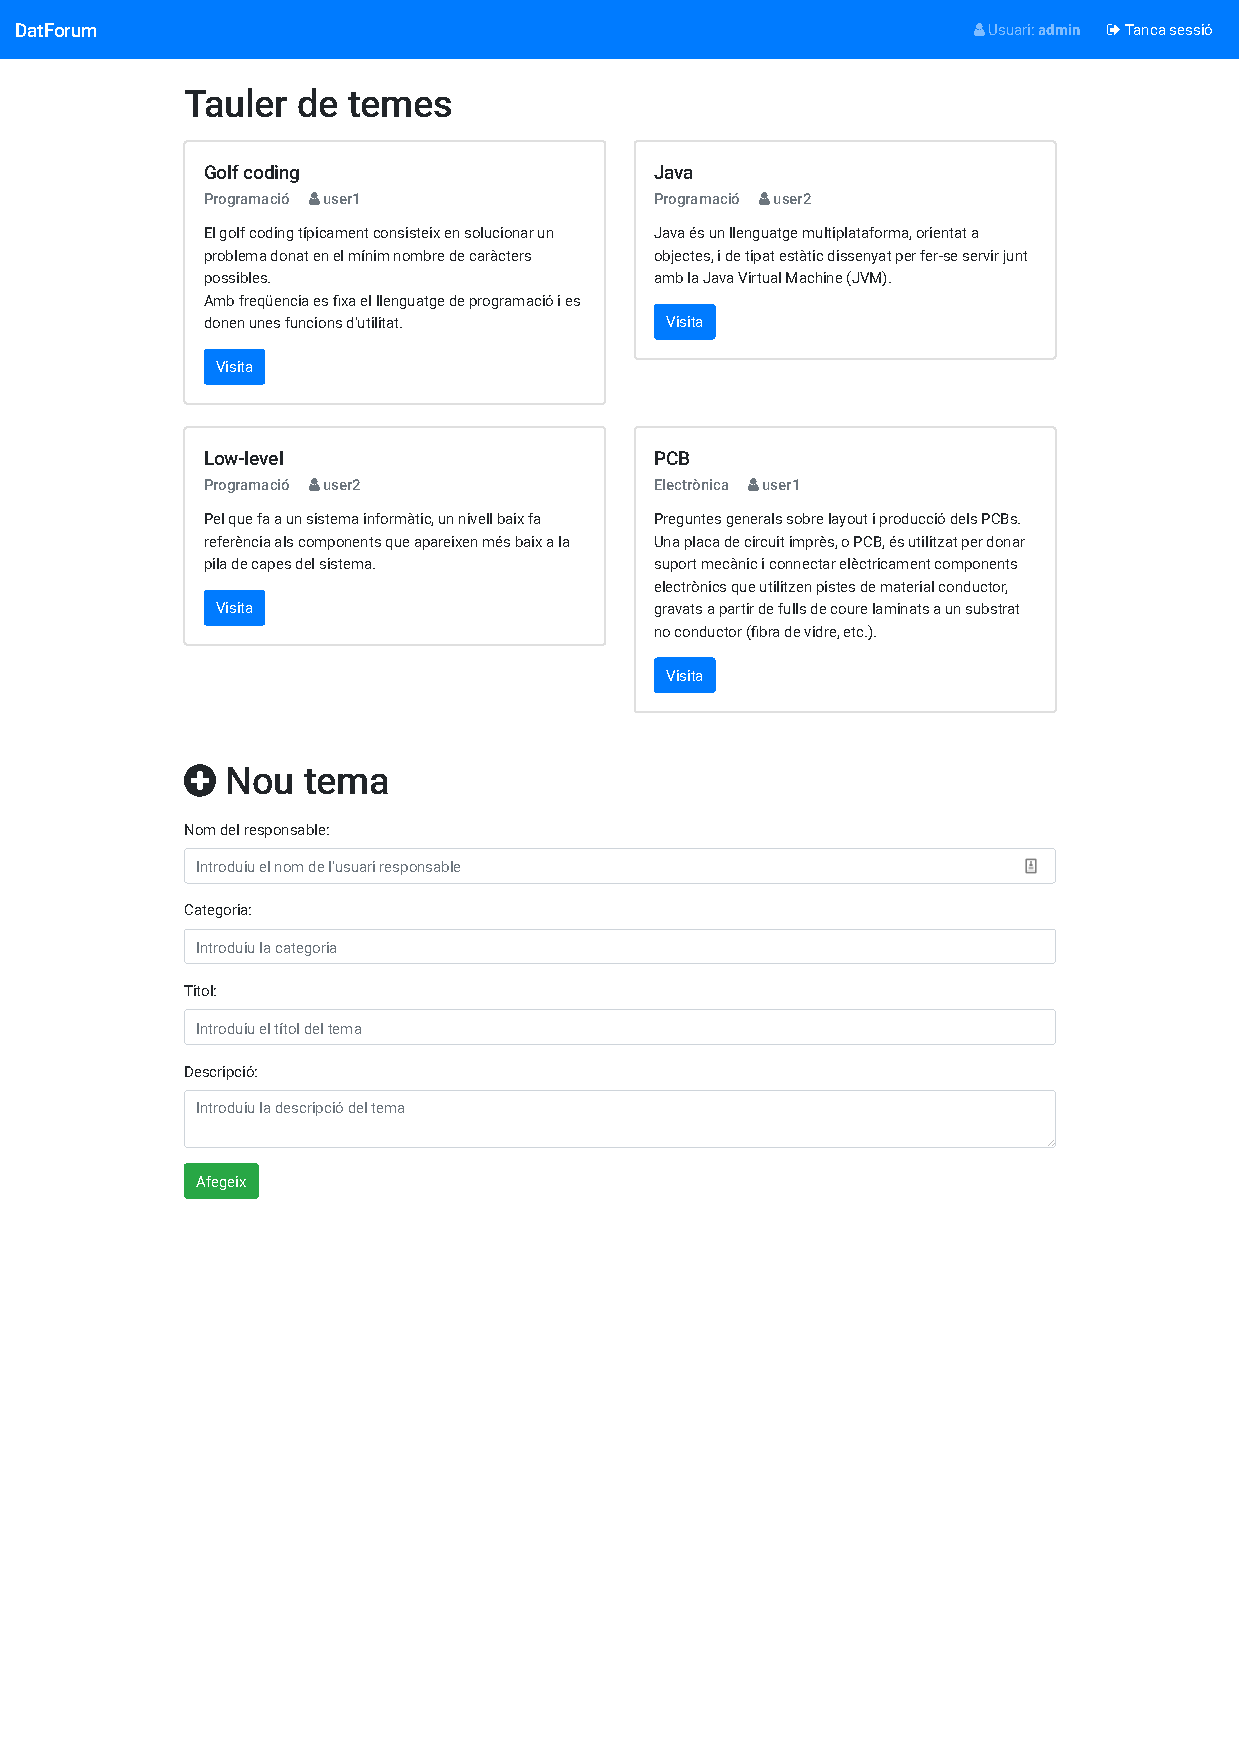
\includegraphics[trim={0 8.2cm 0 0}, clip, width=.98\columnwidth, cframe=gray]{screens/home_admin.pdf}
\caption{\label{fig:home_admin} Vista principal (\emph{home}) per al webmaster. }
\end{figure}

Ara comprovem que el formulari funciona i es poden afegir temes.\\
El disseny resultant es pot veure a la figura~\ref{fig:home_admin}.



\clearpage
\section{Vista \emph{question}}

Ara seguirem amb la vista \emph{question}. Farem aquesta primer, ja que és
menys complexa que la vista de tema, que té dos formularis.

\subsection*{Mètode \textsf{GET}}

Creem manualment
una pregunta amb dues respostes a la base de dades. Llavors definim el formulari
per afegir una resposta, qué només consta d'un camp (el text):

\begin{minted}{haskell}
answerForm :: AForm (HandlerFor Forum) Text
answerForm = freq textareaField (withPlaceholder "Introduiu la text de la resposta" "Text") Nothing
\end{minted}

Noteu que en aquest cas el formulari no retorna un \mintinline{haskell}|Answer|
directament; per fer-ho hauriem de saber l'usuari autenticat, la data actual i
l'ID de la pregunta. És més senzill construir aquest \mintinline{haskell}|Answer|
directament en el moment d'afegir la resposta a la base de dades.

A continuació escrivim el codi per al mètode \textsf{GET} de la ruta:

\begin{minted}[highlightlines={5-6}]{haskell}
getQuestionR :: ThemeId -> QuestionId -> HandlerFor Forum Html
getQuestionR tid qid = do
    -- Get model info
    db <- getsSite forumDb
    (theme, question) <- getThemeQuestion tid qid db
    answers <- liftIO $ getAnswerList qid db
    mbuser <- maybeAuthId
    aformw <- generateAFormPost answerForm
    -- Return HTML content
    defaultLayout $ $(widgetTemplFile "src/forum/templates/question.html")
\end{minted}

El codi és molt similar al de la home, es limita a renderitzar el formulari i la vista.
Però en comptes d'obtenir la llista de temes,
obté la llista de respostes de la pregunta, i la pregunta i tema que es visita. Això
últim es fa mitjançant la funció \mintinline{haskell}|getThemeQuestion|:

%getThemeQuestion :: ThemeId -> QuestionId -> ForumDb -> HandlerFor Forum (Theme, Question)
\begin{minted}{haskell}
getThemeQuestion tid qid db = do
    question <- liftChecked $ getQuestion qid db
    unless (qTheme question == tid) notFound
    theme <- liftChecked $ getTheme tid db
    pure (theme, question)
\end{minted}

Aquesta funció obté la pregunta i el tema de la base de dades, però a més comprova
que la pregunta correspon al tema. Si això no és així, llavors la URL és incorrecta
i cal retornar un 404.

%Per últim, el formulari que es renderitza ara és \mintinline{haskell}|answerForm|.

\subsection*{Plantilla}

En primer lloc mostrem la informació i text de la pregunta:

\begin{minted}{html}
<h1 class="mt-3">#{qTitle question}</h2>
<h5 class="text-muted mb-3">
  <i class="fa fa-question-circle"></i>
  Preguntat a <a href="@{ThemeR tid}">#{tTitle theme}</a>
  per #{qUser question} el #{formatPosted (qPosted question)}
</h5>
<p class="lead" style="white-space: pre-line">#{qText question}</p>
\end{minted}

On la funció \mintinline{haskell}|formatPosted| l'hem definit així:

\begin{minted}{haskell}
formatPosted :: UTCTime -> String
formatPosted = formatTime defaultTimeLocale "%Y-%m-%d %H:%M"
\end{minted}

A continuació (abans de tancar el container) mostrem la llista de respostes:

\begin{minted}{html}
<h2 class="mt-4">#{show (length answers)} respostes</h2>
<div>
  $forall{ p <- answers }
  <div class="my-4">
    <div class="card">
      <div class="card-body">
        <h6 class="card-subtitle mb-3 text-muted">
          <span><i class="fa fa-clock-o"></i> #{formatPosted (aPosted (snd p))}</span>
          <span class="mx-3"><i class="fa fa-user"></i> #{aUser (snd p)}</span>
        </h6>
        <p class="lead mb-0" style="white-space: pre-line">#{aText (snd p)}</p>
      </div>
    </div>
  </div>
  $end
</div>
\end{minted}

Com que s'han de poder esborrar preguntes, ficarem
el codi anterior dins un \mintinline{html}|<form>| amb un botó
de submit (que només es mostra si hi ha respostes i l'usuari és leader):

\begin{minted}{html}
<form role="form" method="POST" action="@{QuestionR tid qid}">
  <!-- ... -->

  $if{ null answers }
  $elseif{ maybe False (isLeader theme) mbuser}
  <div class="row">
    <div class="col-sm-12">
      <button type="submit" class="btn btn-danger" name="delete">Elimina respostes</button>
    </div>
  </div>
  $end
</form>
</div>
\end{minted}

...i en cas de que l'usuari sigui un leader, afegirem checkboxes al
prinicpi de cada resposta per seleccionar-les:

\begin{minted}[highlightlines={2}]{html}
<h6 class="card-subtitle mb-3 text-muted">
  $if{ maybe False (isLeader theme) mbuser }<input type="checkbox" name="aid" value="#{fst p}"/>$end
  <span><i class="fa fa-clock-o"></i> #{formatPosted (aPosted (snd p))}</span>
  <span class="mx-3"><i class="fa fa-user"></i> #{aUser (snd p)}</span>
</h6>
\end{minted}

Per últim, en un nou contenidor mostrem el formulari:

\begin{minted}[highlightlines={1, 13}]{html}
$if{ isJust mbuser }
<div class="container my-4">
<h2 class="my-3"><i class="fa fa-plus-circle"></i> Afegeix una resposta</h2>

<form role="form" method="POST" action="@{QuestionR tid qid}">
  <div class="row">
    <div class="col-sm-12">
      ^{aformw}
    </div>
  </div>
  <div class="row">
    <div class="col-sm-12">
      <button type="submit" class="btn btn-success" name="add">Crea</button>
    </div>
  </div>
</form>
</div>
$end
\end{minted}

El codi és pràcticament idèntic al de la secció anterior, però en aquest
cas la condició és simplement que l'usuari estigui autenticat i la ruta
del formulari es diferent.

A més,
s'ha afegit \mintinline{html}|name| als botons de cadascun dels formularis,
per poder saber quin d'ells s'ha enviat.

\begin{figure}
\centering 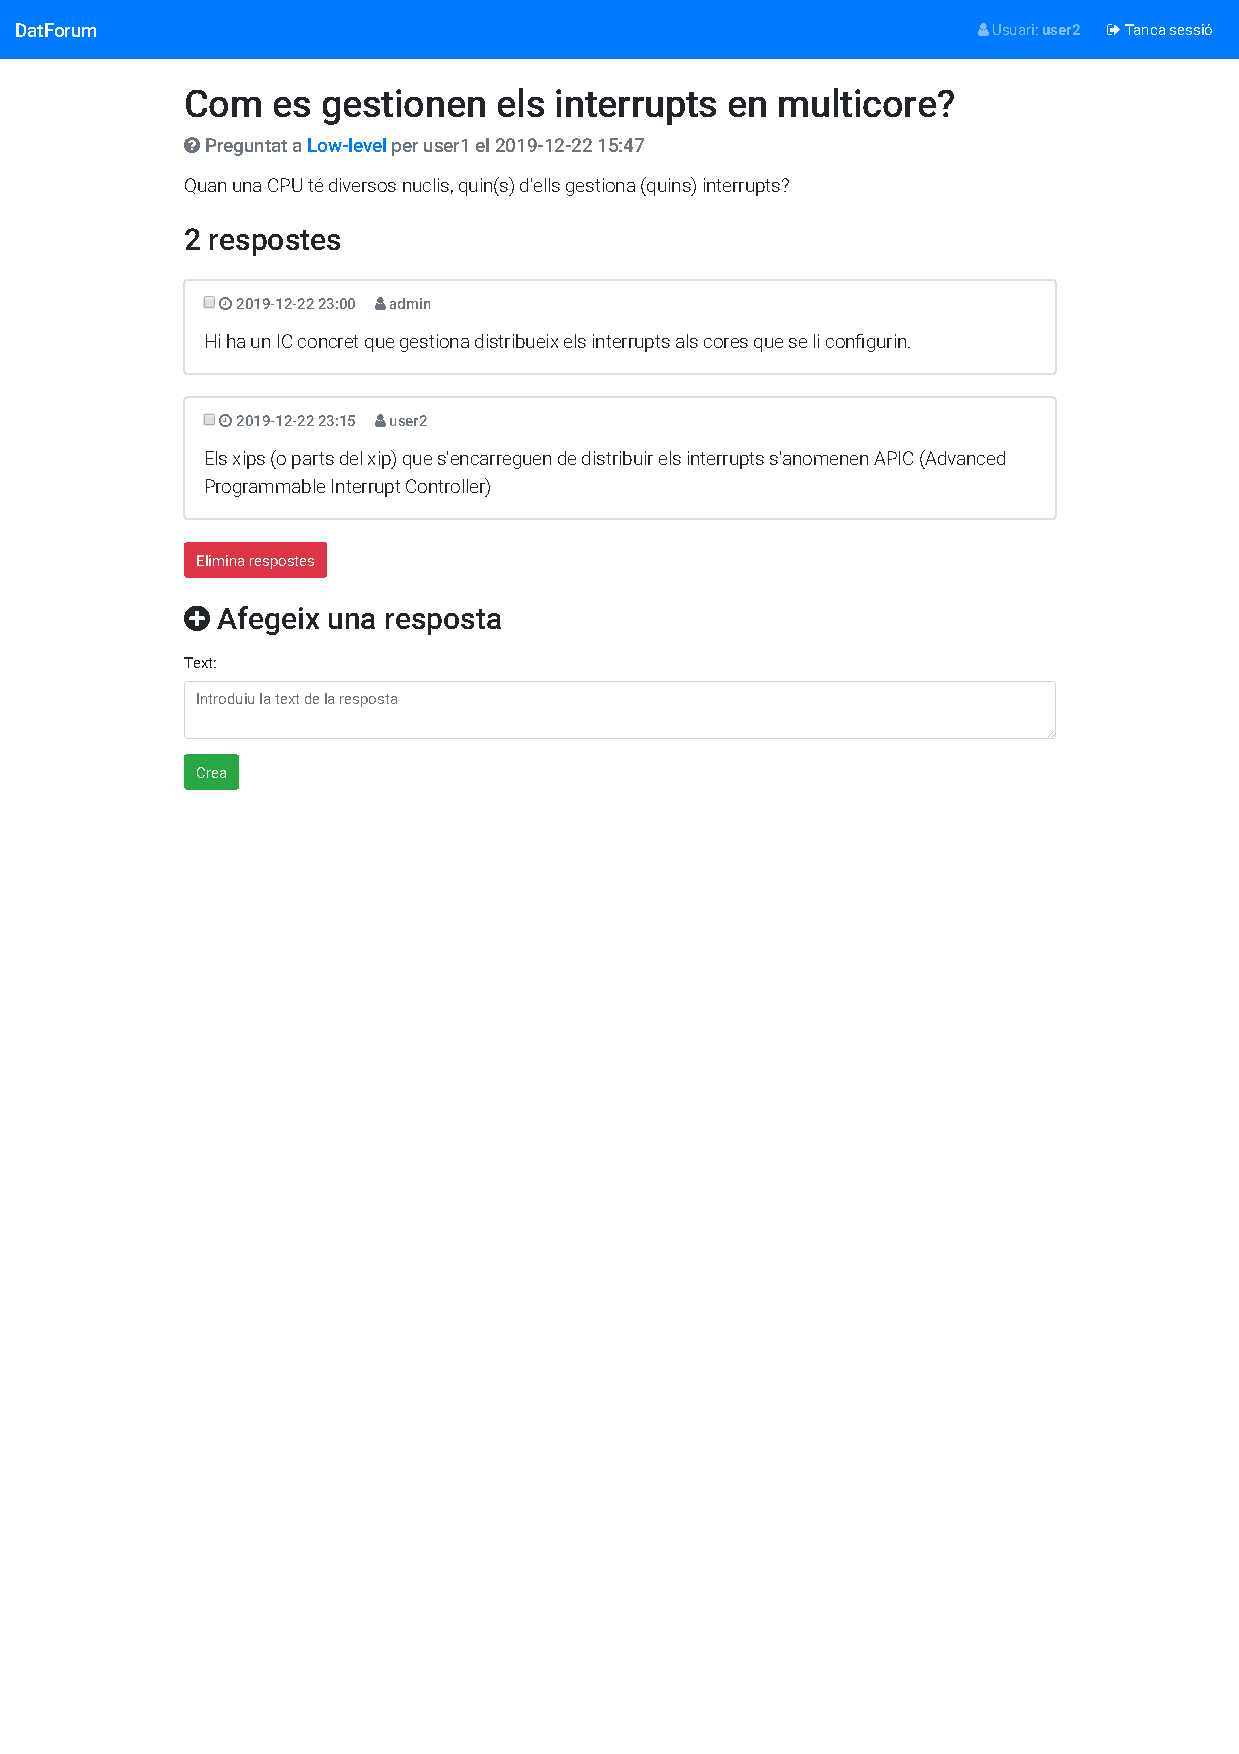
\includegraphics[trim={0 16cm 0 0}, clip, width=.98\columnwidth, cframe=gray]{screens/question_admin.pdf}
\caption{\label{fig:question_admin} Vista d'una pregunta (\emph{question}) per al leader. }
\end{figure}

\begin{figure}
\centering 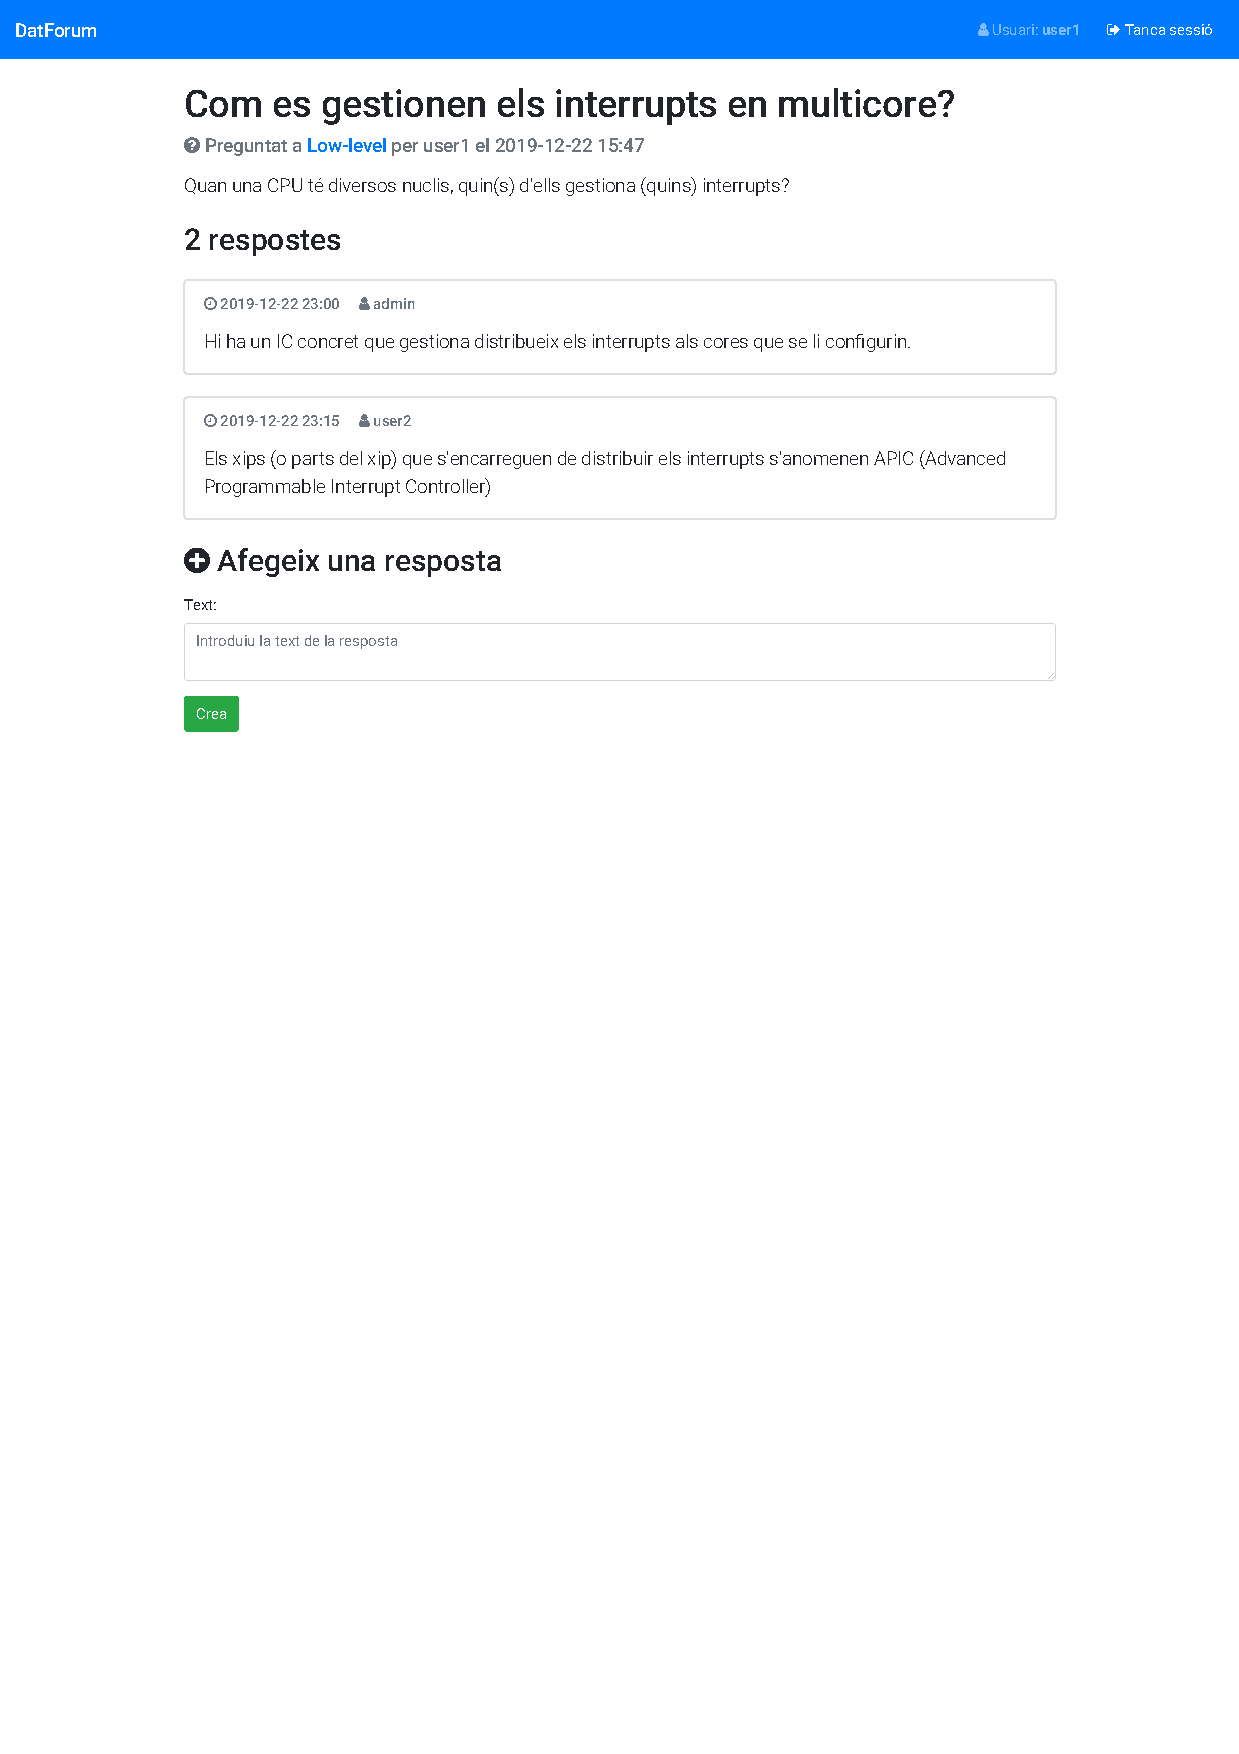
\includegraphics[trim={0 16cm 0 0}, clip, width=.98\columnwidth, cframe=gray]{screens/question_user.pdf}
\caption{\label{fig:question_user} Vista d'una pregunta (\emph{question}) per a un usuari autenticat. }
\end{figure}

\begin{figure}
\centering 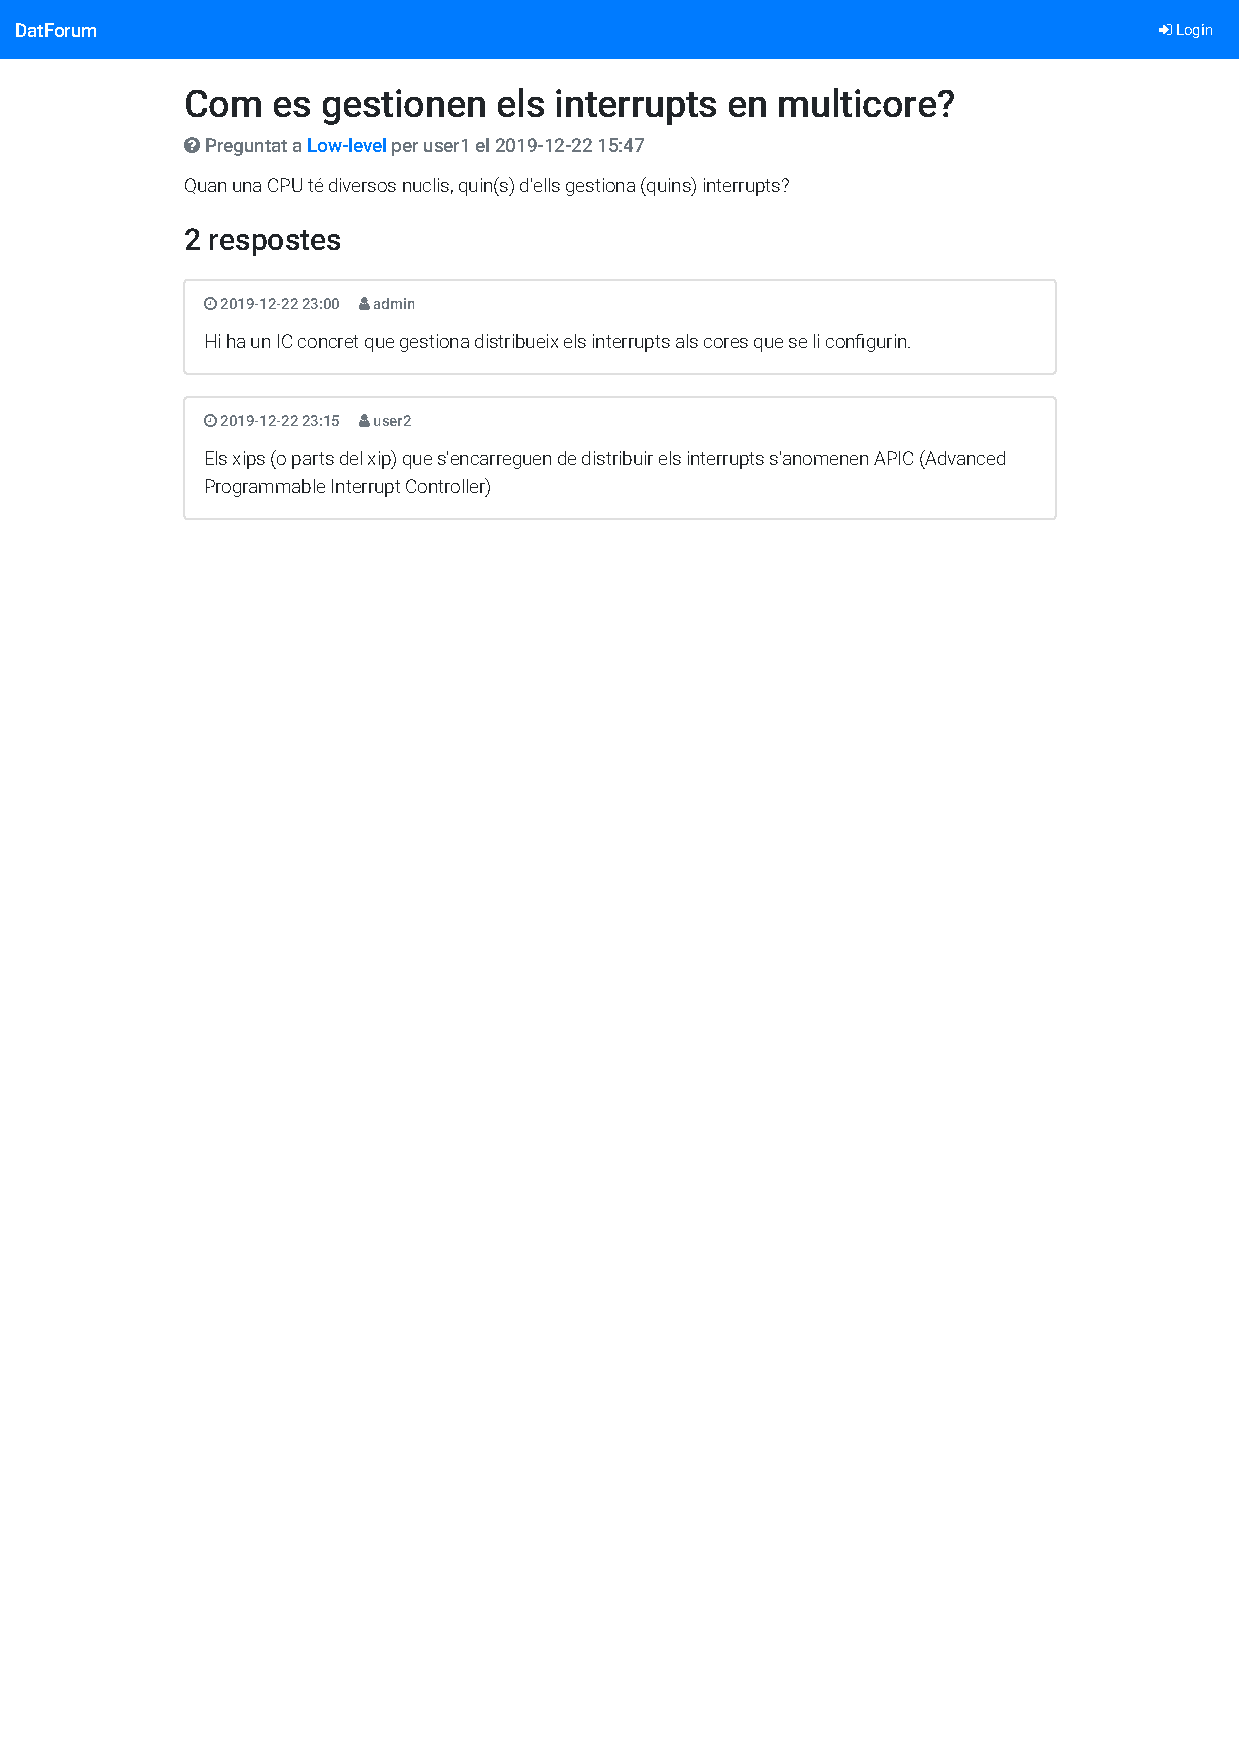
\includegraphics[trim={0 16cm 0 0}, clip, width=.98\columnwidth, cframe=gray]{screens/question_anonymous.pdf}
\caption{\label{fig:question_anonymous} Vista d'una pregunta (\emph{question}) per a un usuari no autenticat. }
\end{figure}

El disseny resultant es pot veure a les figures \ref{fig:question_admin},
\ref{fig:question_user} i \ref{fig:question_anonymous}.

\subsection*{Mètode \textsf{POST}}

Per a implementar el mètode \textsf{POST}, en primer lloc com és habitual
obtindrem la informació de la base de dades i l'usuari que fa la petició:

\begin{minted}{haskell}
postQuestionR :: ThemeId -> QuestionId -> HandlerFor Forum Html
postQuestionR tid qid = do
    user <- requireAuthId
    db <- getsSite forumDb
    (theme, question) <- getThemeQuestion tid qid db
    answers <- liftIO $ getAnswerList qid db
\end{minted}

A continuació mirarem quin dels botons s'ha premut per saber el formulari:

\begin{minted}{haskell}
    deleteForm <- isJust <$> lookupPostParam "delete"
    addForm <- isJust <$> lookupPostParam "add"
    if deleteForm
      then do
        -- formulari 1
      else if addForm then do
        -- formulari 2
      else
        invalidArgs ["delete","add"]
\end{minted}

Llavors, en cas que sigui el primer formulari: s'extreuen les IDs dels
checkboxes que s'han premut, s'eliminen de la base de dades i es redirigeix
l'usuari a la pàgina actual:

\begin{minted}{haskell}
checkBoxes <- lookupPostParams "aid"
let aids = catMaybes ((readMaybe . T.unpack) <$> checkBoxes)
forM_ aids $ \ aid ->
    liftIO $ deleteAnswer aid db
redirectRoute (QuestionR tid qid) []
\end{minted}

En el cas del segon formulari (\mintinline{haskell}|answerForm|), l'executem
per validar els camps introduits. Si tot està bé, es crea la resposta en la
base de dades i es redirigeix. Si no, es renderitza la pàgina amb els errors:

\begin{minted}{haskell}
(aformr, aformw) <- runAFormPost answerForm
case aformr of
    FormSuccess text -> do
        time <- liftIO $ getCurrentTime
        let answer = Answer qid user time text
        liftIO $ addAnswer answer db
        redirectRoute (QuestionR tid qid) []
    _ -> do
        let mbuser = Just user
        defaultLayout $(widgetTemplFile "src/forum/templates/question.html")
\end{minted}

Es comprova que tots els formularis funcionen correctament.



\clearpage
\section{Vista \emph{theme}}

\subsection*{Mètode \textsf{GET}}

Primer creem manualment quatre temes a la base de dades. Llavors hem de definir
els dos formularis que es renderitzaran a la vista: el de modificar el tema,
i el d'afegir una pregunta.

Respecte al de modificar el tema, és més senzill modificar \mintinline{haskell}|themeForm|
(veure secció~\ref{sec:form-category})
perquè accepti un \mintinline{haskell}|Maybe Theme| i el faci servir per als
valors per defecte dels camps. Per fer-ho, només hem de fer que aquests
valors per defecte siguin \mintinline{haskell}|(camp <$> theme)| en comptes
de \mintinline{haskell}|Nothing|:

\begin{minted}{haskell}
themeForm :: Maybe Theme -> AForm (HandlerFor Forum) Theme
themeForm theme =
    Theme <$> maybe
                (freq (checkM checkUserExists textField)
                (withPlaceholder "Introduiu el nom de l'usuari responsable" "Nom del responsable")
                Nothing)
              pure (tLeader <$> theme)
          <*> freq textField (withPlaceholder "Introduiu la categoria" "Categoria") (tCategory <$> theme)
          <*> freq textField (withPlaceholder "Introduiu el títol del tema" "Titol") (tTitle <$> theme)
          <*> freq textareaField (withPlaceholder "Introduiu la descripció del tema" "Descripció") (tDescription <$> theme)
\end{minted}

Observeu que per al camp del leader el que es fa és mostrar-lo
només si \mintinline{haskell}|theme| no està present, en cas
contrari no es deixa modificar-lo (es fa servir el valor existent).

Llavors, reemplacem tots els usos de \mintinline{haskell}{themeForm} per
\mintinline{haskell}{themeForm Nothing}, i per al formulari de modificació
farem servir \mintinline{haskell}{themeForm $ Just theme}.

Respecte al formulari d'afegir una pregunta, aquest té dos camps que
retornarem dins una tupla:

\begin{minted}{haskell}
questionForm :: AForm (HandlerFor Forum) (Text, Text)
questionForm =
    (,) <$> freq textField (withPlaceholder "Introduiu l'assumpte de la pregunta" "Assumpte") Nothing
        <*> freq textareaField (withPlaceholder "Introduiu el text de la pregunta" "Text") Nothing
\end{minted}

Ja podem escriure el mètode \textsf{GET}, que és molt similar
a l'anterior, excepte que renderitzem tots dos formularis:

\begin{minted}{haskell}
getThemeR :: ThemeId -> HandlerFor Forum Html
getThemeR tid = do
    -- Get model info
    db <- getsSite forumDb
    theme <- liftChecked $ getTheme tid db
    questions <- liftIO $ getQuestionList tid db
    mbuser <- maybeAuthId
    tformw <- generateAFormPost (themeForm $ Just theme)
    qformw <- generateAFormPost questionForm
    -- Return HTML content
    defaultLayout $ $(widgetTemplFile "src/forum/templates/theme.html")
\end{minted}

\subsection*{Plantilla}

Comencem mostrant el nom del tema i la descripció:

\begin{minted}{html}
<h1 class="my-3">#{tTitle theme}</h2>
<p class="lead" style="white-space: pre-line">#{tDescription theme}</p>
\end{minted}

A continuació mostrem les preguntes en cards, com es fa en la home:

\begin{minted}{html}
<div class="row row-cols-1 row-cols-md-2">
  $forall{ p <- questions }
  <div class="col mb-4">
    <div class="card">
      <div class="card-body">
        <h5 class="card-title">
          #{qTitle (snd p)}
        </h5>
        <h6 class="card-subtitle mb-3 text-muted">
          <span><i class="fa fa-clock-o"></i> #{formatPosted (qPosted (snd p))}</span>
          <span class="mx-3"><i class="fa fa-user"></i> #{qUser (snd p)}</span>
        </h6>
        <p class="card-text" style="white-space: pre-line">#{qText (snd p)}</p>
        <a href="@{QuestionR tid (fst p)}" class="btn btn-primary">Visita</a>
      </div>
    </div>
  </div>
  $end
</div>
\end{minted}

Igual que en la secció anterior, per tal de poder esborrar preguntes,
movem aquest bloc dins un un \mintinline{html}|<form>| amb un botó
que només es mostra si hi ha preguntes i l'usuari és leader:

\begin{minted}{html}
<form role="form" method="POST" action="@{ThemeR tid}">
  <div class="row row-cols-1 row-cols-md-2">
    <!-- ... -->
  </div>

  $if{ null questions }
  <p>Encara no hi ha preguntes.</p>
  $elseif{ maybe False (isLeader theme) mbuser}
  <div class="row">
    <div class="col-sm-12">
      <button type="submit" class="btn btn-danger" name="delete">Elimina preguntes</button>
    </div>
  </div>
  $end
</form>
</div>
\end{minted}

I afegim checkboxes a cada pregunta per seleccionar-la:

\begin{minted}[highlightlines={2}]{html}
<h5 class="card-title">
  $if{ maybe False (isLeader theme) mbuser }<input type="checkbox" name="qid" value="#{fst p}"/>$end
  #{qTitle (snd p)}
</h5>
\end{minted}

A continuació, renderitzem el formulari d'afegir una pregunta
(si l'usuari està autenticat) i el de modificar el tema (si l'usuari és leader):

\begin{minted}{html}
$if{ isJust mbuser }
<div class="container my-4">
<h2 class="my-3"><i class="fa fa-plus-circle"></i> Crea una nova pregunta</h2>

<form role="form" method="POST" action="@{ThemeR tid}">
  <div class="row">
    <div class="col-sm-12">
      ^{qformw}
    </div>
  </div>
  <div class="row">
    <div class="col-sm-12">
      <button type="submit" class="btn btn-success" name="add">Crea</button>
    </div>
  </div>
</form>

</div>
$end

$if{ maybe False (isLeader theme) mbuser }
<div class="container my-4">
<h2 class="my-3"><i class="fa fa-pencil"></i> Modifica el tema</h2>

<form role="form" method="POST" action="@{ThemeR tid}">
  <div class="row">
    <div class="col-sm-12">
      ^{tformw}
    </div>
  </div>
  <div class="row">
    <div class="col-sm-12">
      <button type="submit" class="btn btn-primary" name="modify">Modifica</button>
    </div>
  </div>
</form>

</div>
$end
\end{minted}

Igual que en la secció anterior, s'ha afegit \mintinline{html}|name| als botons
per diferenciar quins dels tres formularis s'ha enviat.

\begin{figure}
\centering 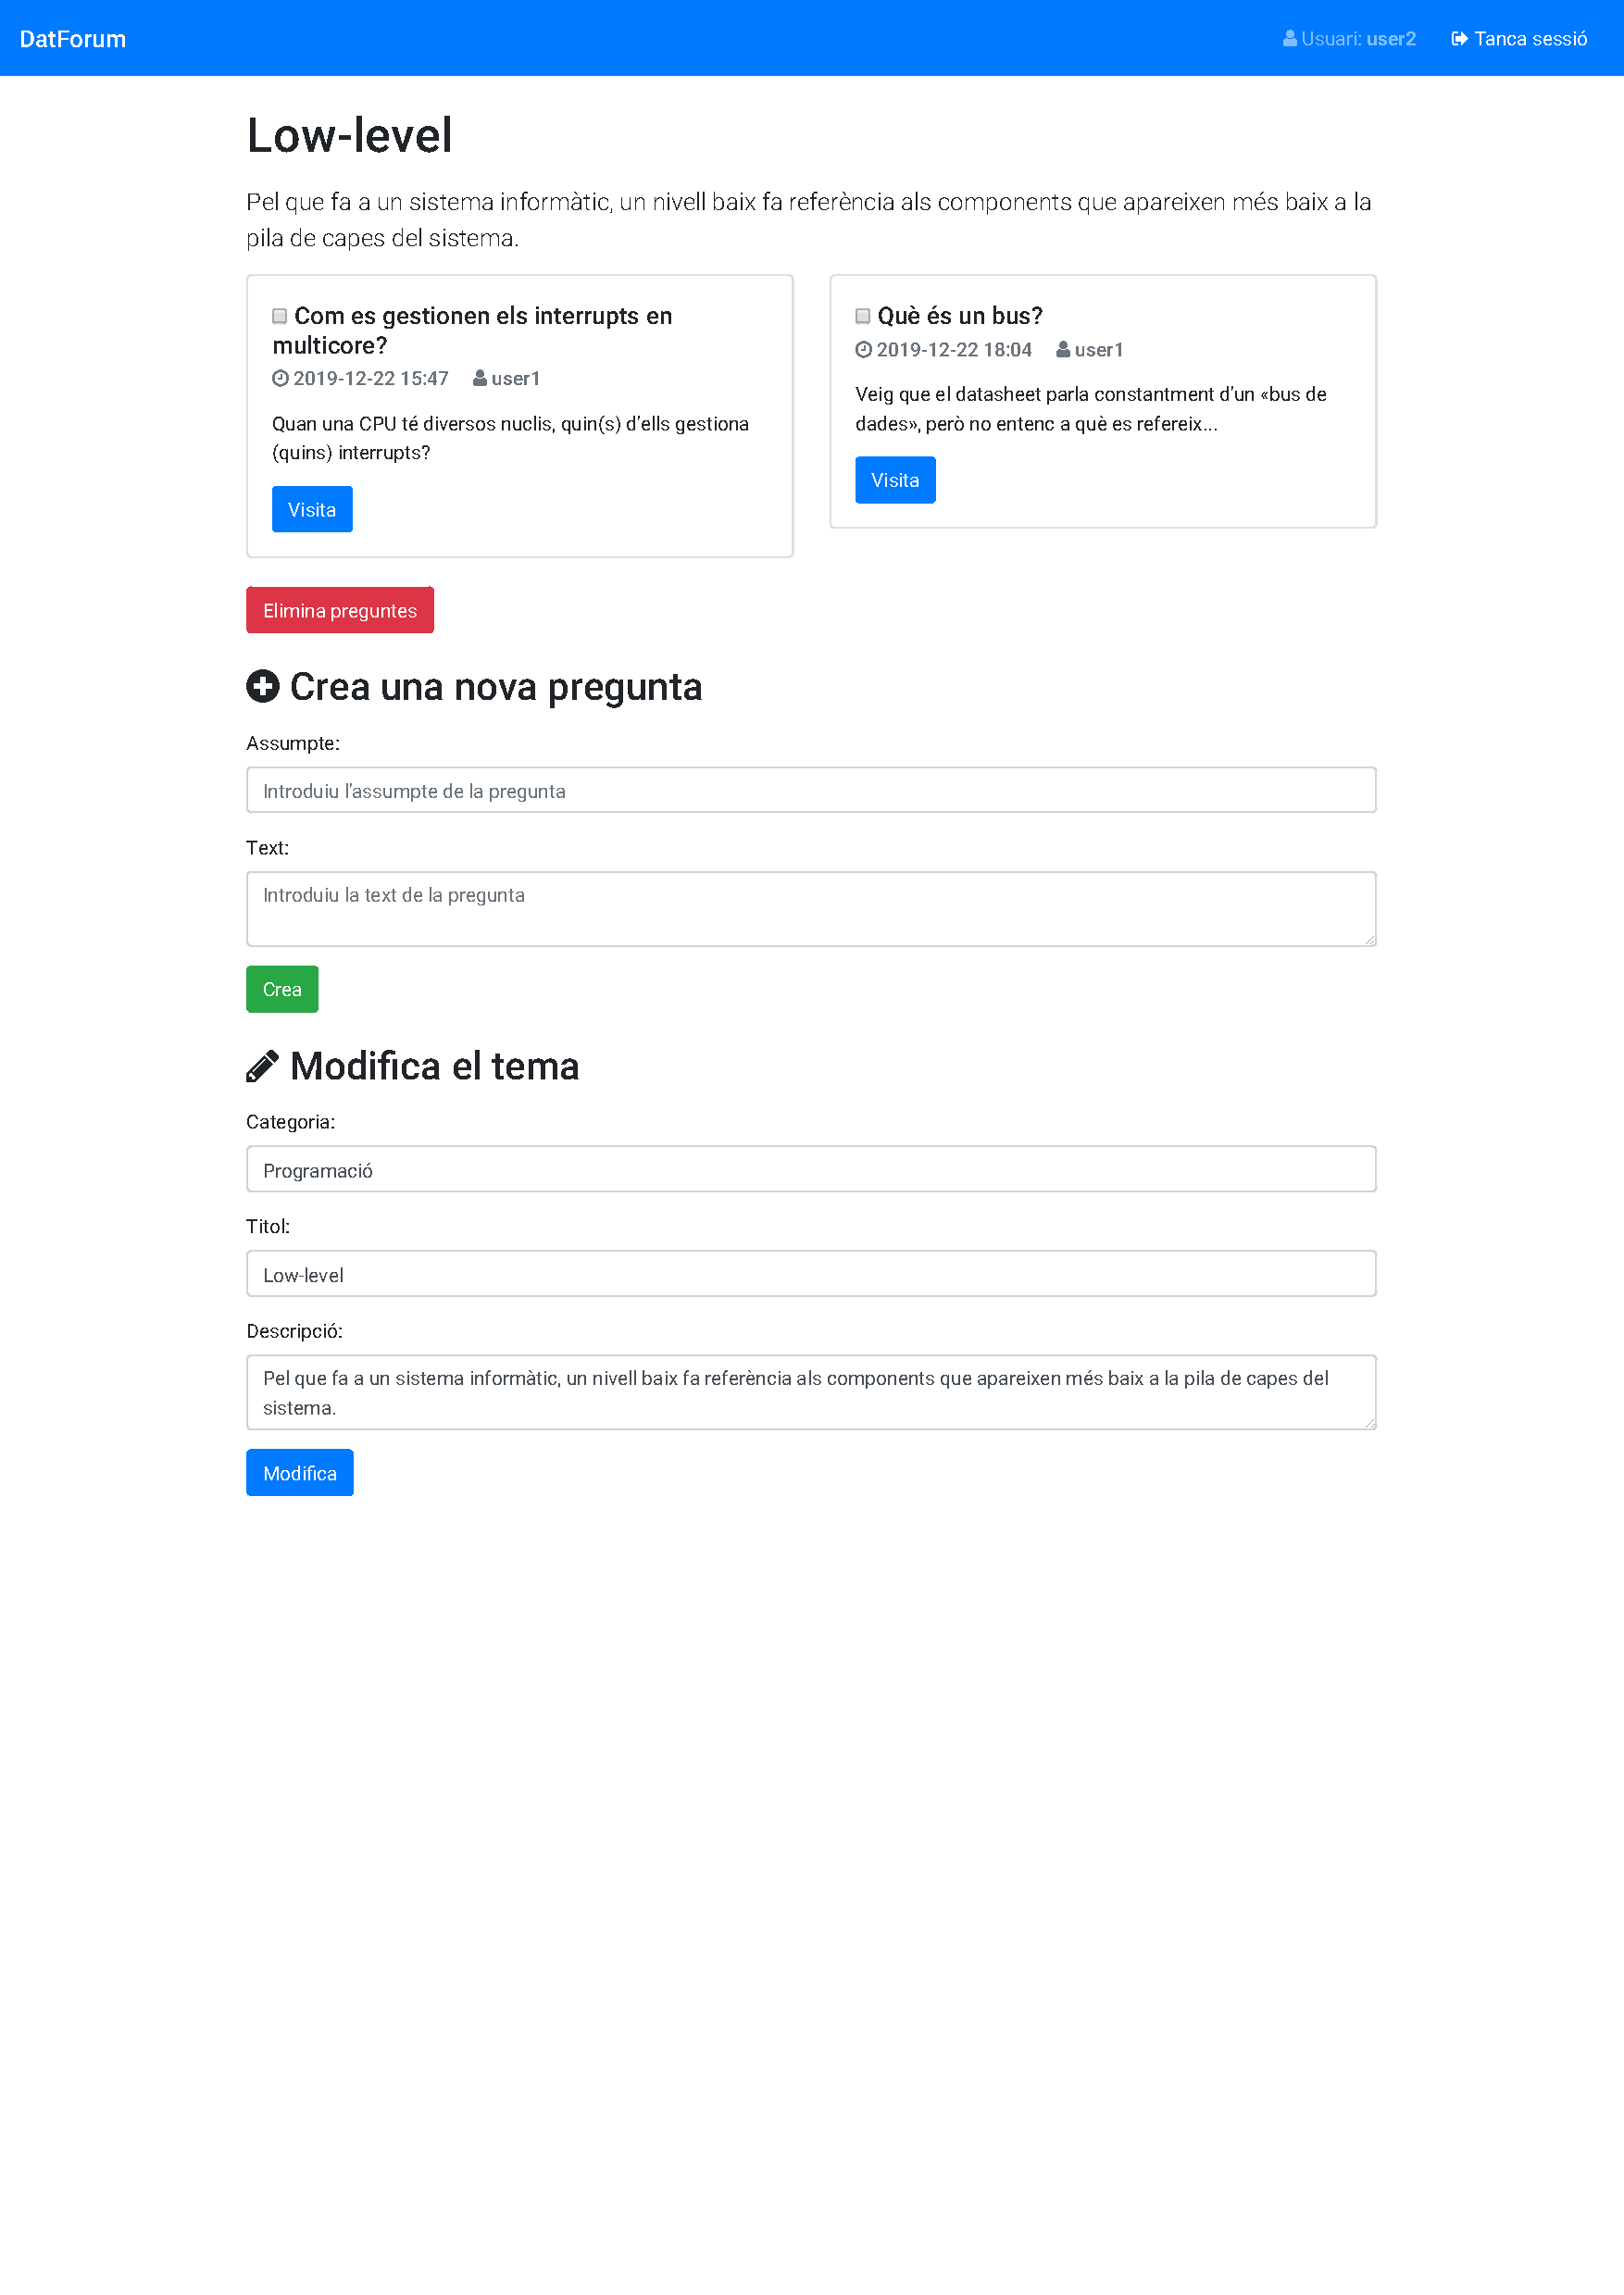
\includegraphics[trim={0 13.4cm 0 0}, clip, width=.98\columnwidth, cframe=gray]{screens/theme_admin.pdf}
\caption{\label{fig:theme_admin} Vista d'un tema (\emph{theme}) per al leader. }
\end{figure}

El disseny resultant es pot veure a la figura~\ref{fig:theme_admin}.

\subsection*{Mètode \textsf{POST}}

L'estructura del mètode \textsf{POST} és molt similar a la de la secció
anterior, obtindrem la informació i discriminarem entre els tres formularis
possibles:

\begin{minted}{haskell}
postThemeR :: ThemeId -> HandlerFor Forum Html
postThemeR tid = do
    user <- requireAuthId
    db <- getsSite forumDb
    theme <- liftChecked $ getTheme tid db
    questions <- liftIO $ getQuestionList tid db
    modifyForm <- isJust <$> lookupPostParam "modify"
    deleteForm <- isJust <$> lookupPostParam "delete"
    addForm <- isJust <$> lookupPostParam "add"
    if modifyForm
      then do
        -- formulari 1
      else if deleteForm then do
        -- formulari 2
      else if addForm then do
        -- formulari 3
      else
        invalidArgs ["modify","delete","add"]
\end{minted}

Pel cas de modificació del tema, com hem fet abans, validem els camps del
formulari. Si estan bé, es modifica el tema a la base de dades i es redirigeix.
Sino es torna a renderitzar la pàgina, però abans cal renderitzar també l'altre
formulari:

\begin{minted}{haskell}
(tformr, tformw) <- runAFormPost (themeForm $ Just theme)
case tformr of
    FormSuccess newtheme -> do
        liftIO $ updateTheme tid newtheme db
        redirectRoute (ThemeR tid) []
    _ -> do
        qformw <- generateAFormPost questionForm
        let mbuser = Just user
        defaultLayout $(widgetTemplFile "src/forum/templates/theme.html")
\end{minted}

Pel cas d'eliminació, de forma també similar a abans, s'obtenen els IDs dels
\emph{checkboxes} marcats, s'eliminen de la base de dades i es redirigeix:

\begin{minted}{haskell}
checkBoxes <- lookupPostParams "qid"
let qids = catMaybes ((readMaybe . T.unpack) <$> checkBoxes)
forM_ qids $ \ qid ->
    liftIO $ deleteFullQuestion qid db
redirectRoute (ThemeR tid) []
\end{minted}

Pel cas d'afegir una pregunta se segueix un procediment similar al primer cas:

\begin{minted}{haskell}
(qformr, qformw) <- runAFormPost questionForm
case qformr of
    FormSuccess (title, text) -> do
        time <- liftIO $ getCurrentTime
        let question = Question tid user time title text
        qid <- liftIO $ addQuestion question db
        redirectRoute (QuestionR tid qid) []
    _ -> do
        tformw <- generateAFormPost (themeForm $ Just theme)
        let mbuser = Just user
        defaultLayout $(widgetTemplFile "src/forum/templates/theme.html")
\end{minted}

Comprovem que tots els formularis funcionen correctament.


\clearpage
\section{Comprovacions de seguretat}

Cal observar que, a banda de comprovar que l'usuari estigui autenticat,
els mètodes \textsf{POST} no verifiquen que l'usuari sigui webmaster o
leader en les operacions que ho requereixen. Això és el que afegirem ara.

En primer lloc, al mòdul \mintinline{haskell}|Found|, definirem funcions
d'utilitat que comproven els permisos de l'usuari, denegant la petició si
no es compleixen:

\begin{minted}{haskell}
requireAdmin :: MonadHandler m => UserId -> m ()
requireAdmin u =
    unless (isAdmin u) (permissionDenied "User is not admin")

requireLeader :: MonadHandler m => Theme -> UserId -> m ()
requireLeader t u =
    unless (isLeader t u) (permissionDenied "User is not leader")
\end{minted}

Ara només cal que fem servir aquestes funcions en els handlers.
En el de la home:

\begin{minted}[highlightlines={4}]{haskell}
postHomeR = do
    user <- requireAuthId
    db <- getsSite forumDb
    requireAdmin user
    (tformr, tformw) <- runAFormPost themeForm
    case tformr of
        -- ...
\end{minted}

En el de la vista de tema:

\begin{minted}[highlightlines={7,12}]{haskell}
postThemeR tid = do
    user <- requireAuthId
    db <- getsSite forumDb
    -- ...
    if modifyForm
      then do
        requireLeader theme user
        (tformr, tformw) <- runAFormPost (themeForm $ Just theme)
        case tformr of
            -- ...
      else if deleteForm then do
        requireLeader theme user
        checkBoxes <- lookupPostParams "qid"
        -- ...
      else if addForm then do
        (qformr, qformw) <- runAFormPost questionForm
        case qformr of
            -- ...
      else
        invalidArgs ["modify","delete","add"]
\end{minted}

En el de la vista de pregunta:

\begin{minted}[highlightlines={7}]{haskell}
postQuestionR tid qid = do
    user <- requireAuthId
    db <- getsSite forumDb
    -- ...
    if deleteForm
      then do
        requireLeader theme user
        checkBoxes <- lookupPostParams "aid"
        -- ...
      else if addForm then do
        (aformr, aformw) <- runAFormPost answerForm
        case aformr of
            -- ...
      else
        invalidArgs ["delete","add"]
\end{minted}

També cal que, quan s'eliminen preguntes, validem que
pertanyen al tema visitat:

\begin{minted}[highlightlines={4-5}]{haskell}
requireLeader theme user
checkBoxes <- lookupPostParams "qid"
let qids = catMaybes ((readMaybe . T.unpack) <$> checkBoxes)
let valid = fromList $ map fst questions
unless (fromList qids `isSubsetOf` valid) notFound
forM_ qids $ \ qid ->
    liftIO $ deleteFullQuestion qid db
redirectRoute (ThemeR tid) []
\end{minted}

I el mateix quan s'eliminen respostes:

\begin{minted}[highlightlines={4-5}]{haskell}
requireLeader theme user
checkBoxes <- lookupPostParams "aid"
let aids = catMaybes ((readMaybe . T.unpack) <$> checkBoxes)
let valid = fromList $ map fst answers
unless (fromList aids `isSubsetOf` valid) notFound
forM_ aids $ \ aid ->
    liftIO $ deleteAnswer aid db
redirectRoute (QuestionR tid qid) []
\end{minted}

Observeu que en aquest cas només comprovem
que pertanyen a la pregunta visitada. Això és suficient, perquè la funció
\mintinline{haskell}|getThemeQuestion| ja comprova que aquesta pregunta
pertany al tema visitat.

\end{document}
